\documentclass{article}
\usepackage{tikz}

\begin{document}

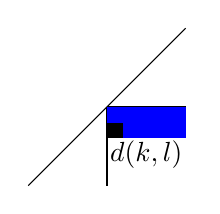
\begin{tikzpicture}[scale=2]
    % Draw the diagonal line
    \draw (0,0) -- (1,1);
    
    % Draw the vertical line
    \draw (0.5,0) -- (0.5,0.5);
    
    % Draw the horizontal line
    \draw (0.5,0.5) -- (1,0.5);
    
    % Draw the blue rectangle
    \fill[blue] (0.5,0.3) rectangle (1,0.5);
    
    % Draw the black square at the bottom left corner of the blue rectangle
    \fill[black] (0.5,0.3) rectangle (0.6,0.4);
    
    % Label the distance
    \node at (0.75,0.2) {$d(k,l)$};
\end{tikzpicture}

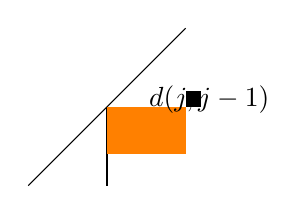
\begin{tikzpicture}[scale=2]
    % Draw the diagonal line
    \draw (0,0) -- (1,1);
    
    % Draw the vertical line
    \draw (0.5,0) -- (0.5,0.5);
    
    % Draw the orange rectangle
    \fill[orange] (0.5,0.2) rectangle (1,0.5);
    
    % Draw the black square at the top right corner of the orange rectangle
    \fill[black] (1,0.5) rectangle (1.1,0.6);
    
    % Label the distance
    \node at (1.15,0.55) {$d(j,j-1)$};
\end{tikzpicture}

\end{document}